\section{The undo tree}
Vim provides multi-level undo.
If you undo a few changes and then make a new change you create a branch in the undo tree.
This text is about moving through the branches.
\localtableofcontentswithrelativedepth{+1}
\subsection{Undo up to a file write}
Sometimes you make several changes, and then discover you want to go back to when you have last written the file.
You can do that with this command:

\begin{Verbatim}[samepage=true]
 :earlier 1f
\end{Verbatim}

The "\verb!f!" stands for "file" here.

You can repeat this command to go further back in the past.
Or use a count different from 1 to go back faster.

If you go back too far, go forward again with:

\begin{Verbatim}[samepage=true]
 :later 1f
\end{Verbatim}

Note that these commands really work in time sequence.
This matters if you made changes after undoing some changes.
It's explained in the next section.

Also note that we are talking about text writes here.
For writing the undo information in a file see |\verb!:h undo-persistence!|.
\subsection{Numbering changes}
\label{Numbering changes}
In section |\hyperref[Undo and Redo]{\texttt{Undo and Redo}}| we only discussed one line of undo/redo.
But it is also possible to branch off.
This happens when you undo a few changes and then make a new change.
The new changes become a branch in the undo tree.

Let's start with the text "one".
The first change to make is to append " too".
And then move to the first 'o' and change it into 'w'.
We then have two changes, numbered 1 and 2, and three states of the text:

\begin{center}
	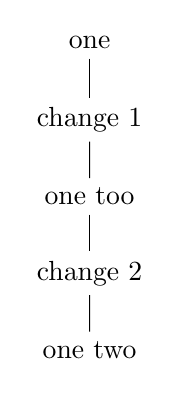
\begin{tikzpicture}[scale=0.65]
		\node[] {one}
		child{node[]{change 1}
		child{node[]{one too}
		child{node[]{change 2}
		child{node[]{one two}
			} } } };
	\end{tikzpicture}
\end{center}

If we now undo one change, back to "one too", and change "one" to "me" we create a branch in the undo tree:

\begin{center}
	\begin{tikzpicture}
		\node[minimum size=2cm] {one}
		child{node[minimum size=2cm]{change 1}
			child{node[minimum size=2cm]{one too}
				child{node[minimum size=2cm]{change 2}
					child{node[minimum size=2cm]{one two}}
				}
				child{node[minimum size=2cm]{change 3}
					child{node[minimum size=2cm]{me too}}
				}
			}
		};
	\end{tikzpicture}
\end{center}

You can now use the |\verb!:h u!| command to undo.
If you do this twice you get to "one".
Use |\verb!:h CTRL-R!| to redo, and you will go to "one too".
One more |\verb!:h CTRL-R!| takes you to "me too".
Thus undo and redo go up and down in the tree, using the branch that was last used.

What matters here is the order in which the changes are made.
Undo and redo are not considered changes in this context.
After each change you have a new state of the text.

Note that only the changes are numbered, the text shown in the tree above has no identifier.
They are mostly referred to by the number of the change above it.
But sometimes by the number of one of the changes below it, especially when moving up in the tree, so that you know which change was just undone.
\subsection{Jumping around the tree}
So how do you get to "one two" now?  You can use this command:

\begin{Verbatim}[samepage=true]
 :undo 2
\end{Verbatim}

The text is now "one two", you are below change 2.
You can use the |\verb!:h :undo!| command to jump to below any change in the tree.

Now make another change: change "one" to "not":

\begin{center}
\begin{tikzpicture}
	\node[minimum size=2cm]{one}
	child{node[minimum size=2cm]{change1}
		child{node[minimum size=2cm]{one too}
			child{node[minimum size=2cm]{one two}
				child{node[minimum size=2cm]{change 4}
					child{node[minimum size=2cm]{not two}}
				}
			}
			child{node[minimum size=2cm]{change 3}
				child{node[minimum size=2cm]{me too}}
			}
		}
	};
\end{tikzpicture}
\end{center}

Now you change your mind and want to go back to "me too".
Use the |\verb!:h g-!| command.
This moves back in time.
Thus it doesn't walk the tree upwards or downwards, but goes to the change made before.

You can repeat |\verb!:h g-!| and you will see the text change:

\begin{Verbatim}[samepage=true]
		me too 
		one two 
		one too 
		one 
\end{Verbatim}

Use |\verb!:h g+!| to move forward in time:

\begin{Verbatim}[samepage=true]
		one 
		one too 
		one two 
		me too 
		not two 
\end{Verbatim}

Using |\verb!:h :undo!| is useful if you know what change you want to jump to.
|\verb!g-!| and |\verb!g+!| are useful if you don't know exactly what the change number is.

You can type a count before |g-| and |\verb!:h g+!| to repeat them.
\subsection{Time travelling}
When you have been working on text for a while the tree grows to become big.
Then you may want to go to the text of some minutes ago.

To see what branches there are in the undo tree use this command:

\begin{Verbatim}[samepage=true]
 :undolist
	number changes  time 
		 3       2  16 seconds ago
		 4       3  5 seconds ago
\end{Verbatim}

Here you can see the number of the leaves in each branch and when the change was made.
Assuming we are below change 4, at "not two", you can go back ten seconds with this command:

\begin{Verbatim}[samepage=true]
 :earlier 10s
\end{Verbatim}

Depending on how much time you took for the changes you end up at a certain position in the tree.
The |\verb!:earlier!| command argument can be "\verb!m!" for minutes, "\verb!h!" for hours and "\verb!d!" for days.
To go all the way back use a big number:

\begin{Verbatim}[samepage=true]
 :earlier 100d
\end{Verbatim}

To travel forward in time again use the |\verb!:later!| command:

\begin{Verbatim}[samepage=true]
 :later 1m
\end{Verbatim}

The arguments are "\verb!s!", "\verb!m!" and "\verb!h!", just like with |\verb!:h :earlier!|.

If you want even more details, or want to manipulate the information, you can use the |\verb!:h undotree()!| function.
To see what it returns:

\begin{Verbatim}[samepage=true]
 :echo undotree()
\end{Verbatim}
\clearpage
